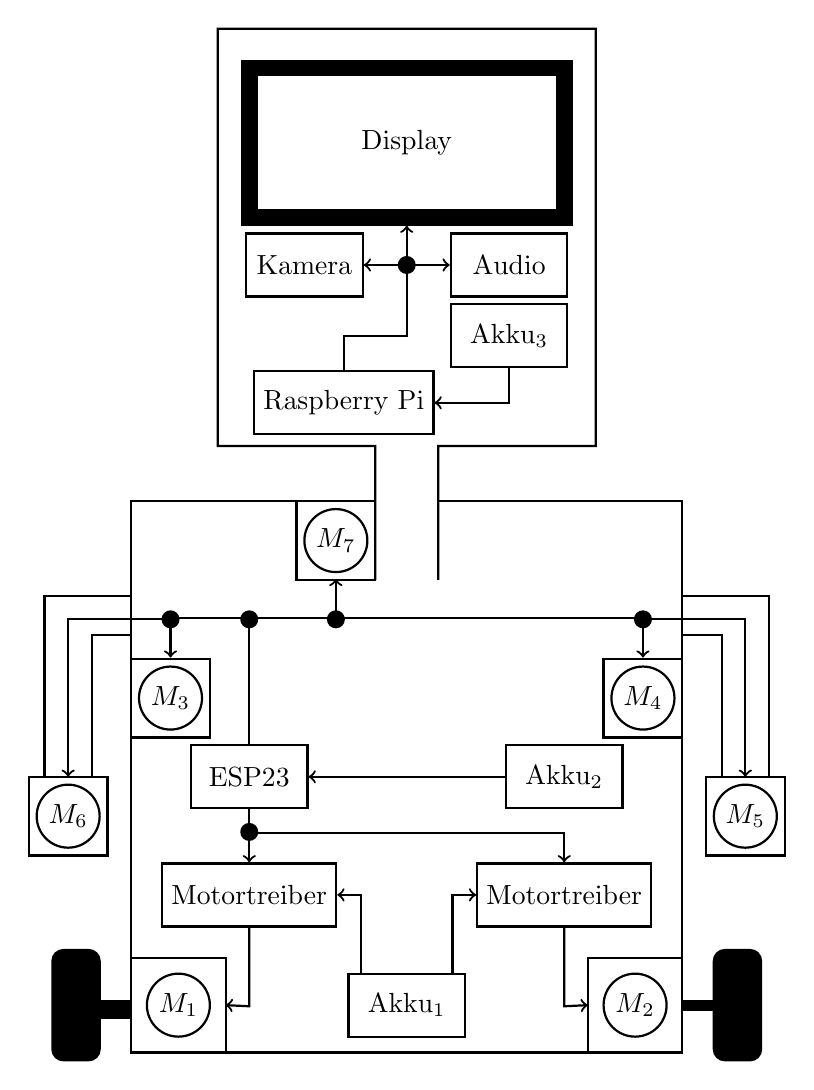
\begin{tikzpicture}[thick, box/.style={
		draw,				
		align=center,
		minimum width=1.48cm,
		minimum height=0.8cm
	}
	]
	
	
	\begin{scope}[shift={(0,0)}] 
		\draw[rounded corners,fill=black]
		(-1,0.6+0.7) rectangle (-0.4,0.6-0.7);
		\draw[line width=4] (0,0.6) -- ++ (-0.4,0);
		%Reifen Rechts
		\draw[rounded corners,fill=black]
		(7+1,0.6+0.7) rectangle (7+0.4,0.6-0.7);
		\draw[line width=4] (7,0.6) -- ++ (+0.4,0);
		
		
		\draw[] (3.5-0.4,7) -- (0,7 )-- (0,0) -- (7,0) -- (7,7) -- (3.5+0.4,7) ;
		%Motoren
		\draw[] (0,0) rectangle (1.2,1.2);
		\draw[] (0.6,0.6) circle (0.4) node[align=center] {$M_1$};
		
		\draw[] (5.8,0) rectangle (7,1.2);
		\draw[] (6.4,0.6) circle (0.4) node[align=center] {$M_2$};
		
		
		
		
		\node[box] (aud)   at (7-2.2,10) {Audio};
		\node[box] (cam)   at (2.2,10) {Kamera};
		\node[box] (rasbe)  at (2.7,8.25)  {Raspberry Pi};
		\node[box] (bat3)   at (7-2.2,9.1) {$\mathrm{Akku}_3$};
		\node[box] (esp)  at (1.5,3.5) {ESP23};
		\node[box] (bat1)   at (3.5,0.6) {$\mathrm{Akku}_1$};
		\node[box] (bat2)   at (5.5,3.5) {$\mathrm{Akku}_2$};
		\node[box]     (M-treL) at (1.5,2) {Motortreiber};
		\node[box]     (M-treR) at (5.5,2) {Motortreiber};
		
		\draw[->] (bat3.south) -- (7-2.2,8.25) --  (rasbe.east);
		\draw[->] (M-treL.south) -- ++ (0,-1) -- (1.2,0.6);
		\draw[->] (M-treR.south) -- ++ (0,-1) -- (5.8,0.6);
		
		\draw[<-] (M-treL.east) -- ++ (0.3,0) -- ++ (0,-1);
		\draw[<-] (M-treR.west) -- ++ (-0.3,0) -- ++ (0,-1);
		
%		\draw[->] (bat2.west) -- (3.5,3.5) --  (rasbe.south);
		\draw[->] (bat2.west) -- (esp.east);
		\draw[->] (rasbe.north) -- (2.7,9.1) -- (3.5,9.1) -- (3.5,10) -- (aud.west);
		\draw[->] (3.5,10) -- (cam.east);
		\draw[->] (3.5,10)-- ++ (0,0.5);
		
		%		\draw[->] (bat1.north) --  (rasbe.south);
		%		\draw[->] (bat1.north) -- ++ (0,2.5) -- (esp.east);
		\draw[->] (esp.south) -- (M-treL.north);
		\draw[->] (esp.south) -- ++ (0,-0.3) -- ++ (4,0) -- (M-treR.north);
		\draw[->] (esp.north) -- ++ (0,1.6) -- ++ (-1,0) -- ++ (0,-0.5);
		\draw[->] (esp.north) -- ++ (0,1.6) -- ++ (5,0) -- ++ (0,-0.5);
		\draw[->] (esp.north) -- ++ (0,1.6) -- ++ (1.1,0) -- ++ (0,0.5);
		
		\draw[->] (0.5,5.5) -- ++ (-1.3,0) -- ++ (0,-2);
		\draw[->] (6.5,5.5) -- ++ (1.3,0) -- ++ (0,-2);
		%Knotenpunkte
		\draw[fill=black] (3.5,10) circle (0.1); %resp
		\draw[fill=black] (1.5,5.5) circle (0.1);
		\draw[fill=black] (1.5,2.8) circle (0.1);
		\draw[fill=black] (2.6,5.5) circle (0.1);
		\draw[fill=black] (0.5,5.5) circle (0.1);
		\draw[fill=black] (6.5,5.5) circle (0.1);	
		
		\draw[] (7.3,3.5) rectangle (8.3,2.5);
		\draw[] (7.8,3) circle (0.4) node[align=center] {$M_5$};
		\draw[] (-0.3,3.5) rectangle (-1.3,2.5);
		\draw[] (-0.8,3) circle (0.4) node[align=center] {$M_6$};
		
		%arm Rechts
		\draw[]
		(0,5.8) -- (-0.8-0.3,5.8) -- ++ (0,-2.3) -- ++ (0.6,0) -- ++ (0,1.8) -- ++ (0.5,0);
		%arm Links
		\draw[]
		(7,5.8) -- (7.8+0.3,5.8) -- ++ (0,-2.3) -- ++ (-0.6,0) -- ++ (0,1.8) -- ++ (-0.5,0);
		
		\draw[line width=4] (0,0.5) -- ++ (-0.81,0);
	\end{scope}
	
	\begin{scope}[shift={(0,+5)}] 
		%Arne
		\draw[] (0,0) rectangle (1,-1);
		\draw[] (0.5,-0.5) circle (0.4) node[align=center] {$M_3$};
		
		\draw[] (6,0) rectangle (7,-1);
		\draw[] (6.5,-0.5) circle (0.4) node[align=center] {$M_4$};
		
%		\draw[] (8,0) rectangle (9,1);
%		\draw[] (6.5,0.5) circle (0.4) node[align=center] {$M_4$};
		
%		\draw[]
%		(-0.8,0.5) rectangle (-0.2,0.6-2);
%		\draw[line width=4] (0,0.5) -- ++ (-0.81,0);
		%Reifen Rechts
%		\draw[]
%		(7+0.8,0.5) rectangle (7+0.3,0.6-2);
%		\draw[line width=4] (7,0.5) -- ++ (+0.81,0);
	\end{scope}
	
	
	\begin{scope}[shift={(0,0)}] 
		%	Kopf	♫
		\draw[] (3.5-0.4,6) -- ++ (0,1.7) -- ++ (-2,0) -- ++ (0,5.3) -- ++ (4+0.8,0) -- ++ (0,-5.3) -- ++ (-2,0)-- (3.5+0.4,6);
		
		\draw[] (3.5-1.4,6) rectangle (3.5-1.4+1,7);
		\draw[] (3.5-1.4+0.5,6.5) circle (0.4) node[align=center] {$M_7$};
		
		%Display
		\draw[line width=6pt]
		(1.5,10.6) rectangle (5.5,12.5)
		node[midway, align=center] {Display};
		
		
	\end{scope}
	
	
	%		\node[boxleft] (req)  at (0,8)  {Anforderungen\\(Systemanforderungen)};
	%		\node[boxleft] (sys)  at (1,6) {Systementwurf\\(Architektur)};
	%		\node[boxleft] (sw)   at (2,4) {Detailentwurf\\(HW/SW-Design)};
	%		\node[box]     (impl) at (4.5,1.6) {Implementierung\\(Codierung/Integration)};
	%		
	%		\node[boxright] (unit) at (7,4) {Modultest\\(Unit Tests)    };%\\(Unit Test)};
%		\node[boxright] (int)  at (8,6) {Integrationstest\\(Systemintegration)};
%		\node[boxright] (acc)  at (9,8) {Abnahme/Validierung\\(Akzeptanztest)};
%		
%		\draw[->] (req.south) -- (sys.north);
%		\draw[->] (sys.south) -- (sw.north);
%		\draw[->] (sw.south)  -- (impl.north);
%		
%		\draw[->] (impl.north) -- (unit.south);
%		
%		\draw[->] (unit.north) -- (int.south);
%		\draw[->] (int.north)  -- (acc.south);
%		
%		\draw[dashed] (sw.east)  -- (unit.west);
%		\draw[dashed] (sys.east) -- (int.west);
%		\draw[dashed] (req.east) -- (acc.west);
%		
%		\node[align=center] at (1.8,0.5) {\footnotesize Entwicklungsphase};
%		\node[align=center] at (8.4,0.5) {\footnotesize Test- und Validierungsphase};







\end{tikzpicture}